\documentclass[a4paper]{article}

\usepackage[utf8]{inputenc}
\usepackage[ngerman]{babel}
\usepackage[autostyle=true,german=quotes]{csquotes}
\usepackage{amsmath}
\usepackage{amsfonts}
\usepackage{amssymb}
\usepackage{graphicx}
\usepackage{longtable}
\usepackage{rotating}
\usepackage{hvfloat}
\usepackage{tabularx}
\usepackage[left=2.5cm,right=2.5cm,top=2.5cm,bottom=2.5cm]{geometry}
\usepackage[colorlinks, linkcolor = black, citecolor = black, filecolor = black, urlcolor = blue]{hyperref}
\author{Sebastian Gottwald, Simon Bordewisch}
\title{Text-Mining Praktikumsbericht}
\date{4. Februar 2016}
\begin{document}
\begin{titlepage}
\maketitle
\end{titlepage}

\section{Einleitung}
	Im Rahmen des Moduls Text-Mining hatten wir die Aufgabe einen Klassifikator für den Stanford Named Entity Recognizer (Stanford NER) zu erstellen.
	Als Datengrundlage stand uns ein von Studenten erstelltes Programm zur Verfügung, welches eine kategorisierte Liste von Titeln der deutschen Wikipedia erzeugt.
	Unsere Aufgabe war es diese Daten aufzubereiten und, anhand von Wikipediaartikeln aus einem XML-Dump, Trainingsdaten für den Stanford NER Klassifikator zu erstellen, welcher Personen-, Organisations- und Ortsnamen erkennt.
	\\\\
	Der Stanford NER ist eine Java-Implementation eines Named Entity Recognizers (NER).
	Ein NER markiert Wort-Sequenzen in einem Text, welche bestimmte Kategorien repräsentieren (z.B. Personen, Orte, Organisationen oder auch Gene und Proteine).
\section{Methodik und Vorgehen}
	\subsection{Auswahl der Vergleichsdaten}
		Insgesamt standen fünf verschiedene Programme des Vorjahrespraktikums zur Verfügung, welche wir als Ausgangsdaten zur Erstellung der Klassifikators nutzen sollten.
		Die Entscheidung fiel auf das Programm, welches auf den Titeln der Wikipediaartikel arbeitet, da dieses eine umfangreiche und nahezu fehlerfreie Liste von Organisationen, sowie Personen- und Ortsnamen liefert.
		Die anderen Programme waren schlecht oder gar nicht dokumentiert, beziehungsweise ohne weiteres Zutun nicht lauffähig.
		Das Programm ''WIKI\_ORG'' arbeitet zum Beispiel auf einer Datenbank, welche nicht mehr vorhanden ist und im Programm ''WIKI\_ORT'' fehlten zusätzliche Abhängigkeiten.

	\subsection{Extraktion der Wikipedia Artikel}
		Als Datengrundlage zur Erstellung der Trainingsdaten des Klassifikators dient der aktuelle Wikipedia Dump\footnote{''dewiki-latest-pages-articles.xml.bz2''}.
		Zur Extraktion der Daten wurde die StAX-API verwendet, da diese sich für große XML-Datenmengen eignet.
		Bei der Extraktion des Wikipedia-Dumps wurden nur Artikel extrahiert, die sich auf Personen, Orte oder Körperschaften beziehen. Hierfür wurden die in dem XML vorhandenen Bezeichnungen genutzt (bspw. für Personen der Tag ''Typ=p'').
		Zur Bereinigung der extrahierten Artikel wurde das Python-Script ''WikiExtraktor.py''\footnote{Quelle: \url{https://github.com/attardi/wikiextractor}} verwendet, welches den Klartext der Wikipediaartikel im Ordner ''Ergebnisse/AA/wiki\_00'' abspeichert. Dadurch wollten wir eine hohe Dichte an Wörter aus den drei Kategorien erreichen, um möglichst kompakte Trainingsdaten zu erhalten.

	\subsection{Volltextsuche und Tagging}
		Um die Trainingsdaten erstellen zu können, musste zunächst ein Wörterbuch erstellt und der extrahierte Klartext getaggt werden.
		Ziel war es den Klartext so vorzubereiten, dass dieser anschließend in die Form gebracht werden konnte, die für den Standford NER benötigt wird.

		\subsubsection{Erstellung des Wörterbuchs}
			Um ein möglichst gutes Wörterbuch erstellen zu können, mit dem der Tagger arbeiten kann, haben wir uns dazu entschieden die Vergleichsdaten der Titel-Gruppe aufzuarbeiten.
			Die Vergleichsdaten, die alle Körperschaften, Orte und Personen in einer Datei enthielten, wurden von einem Parser\footnote{vgl. package ''parsetitlenorm''} zunächst in die verschiedenen Kategorien aufgeteilt, bereinigt und anschließend in drei verschiedenen Dateien (eine pro Kategorie) im CSV-Format gespeichert.
			Bei der Bereinigung wurden Wörter, die in einer Blacklist stehen, herausgefiltert.
			Ursprünglich sollten hier die Namen der Personen nach Vor- und Nachname getrennt werden. 
			Dies wurde allerdings im späteren Entwicklungsverlauf beim Einlese-Prozess der CSV-Dateien in den Tagger realisiert.

		\subsubsection{Einlesen des Klartextes und Tagging}
			Das package ''mapping'' dient dazu die Klartexte, die zu Trainingszwecken genutzt werden sollen, einzulesen und die Wörter einzeln zu untersuchen. 
			Außerdem werden die Wörter zu markiert, die als ein ''Match'', also eine Übereinstimmung mit dem Wörterbuch, erkannt wurden.
			Die Definition des Matches unterlief dabei mehrere Iterationen.
			Zunächst wurden nur vollständige Übereinstimmungen als Match angesehen.
			Dies lieferte jedoch zu schlechte Ergebnisse, da zum Beispiel gebeugte Namen (z.B. ''Merkels'') nicht erkannt werden.
			Daraufhin wurde die Levenshtein-Distanz zur Berechnung der Ähnlichkeit benutzt, um die obigen Ergebnisse zu verbessern.
			Später wurde das Programm so abgeändert, dass die Ähnlichkeit der Suffixe der Wörter (die letzten drei Buchstaben der Wörter) berechnet wurden, während der Rest des Wortes exakt übereinstimmen muss.
			Für das Ähnlichkeitsmaß wurden die Ergebnisse der obig genannten Gruppen verwendet, welche auf der Levenshtein-Distanz relativ zur Gesamtlänge des Eintrages basiert, sodass die Ähnlichkeit ca. 83\% betragen muss.
			Mit der Implementierung von Gewichtungen, die sowohl die Ähnlichkeit des Eintrags als auch das Fehlen von zum Beispiel der Vornamen (zum Beispeil im Fall des Eintrages ''Angela Merkel'', wenn im Text nur ''Merkel'' vorkommt) gewichtet, liefert das Matching gute Ergebnisse.
			Diese Matchings wurden von dem Programm markiert.
			Hierfür wurden XML-ähnliche Tags verwendet (vgl. Abbildung 1).
			Der daraus resultierende Text mit den Tags wird anschließend in eine Datei geschrieben (Standard: ''Ergebnisse/Mapped.out'').
			Diese ermöglicht durch seine Struktur ein Debugging der Texte, da die XML-Tags den im Wörterbuch gefundenen Match enthalten.
			\begin{figure}[htb]
			\centering
			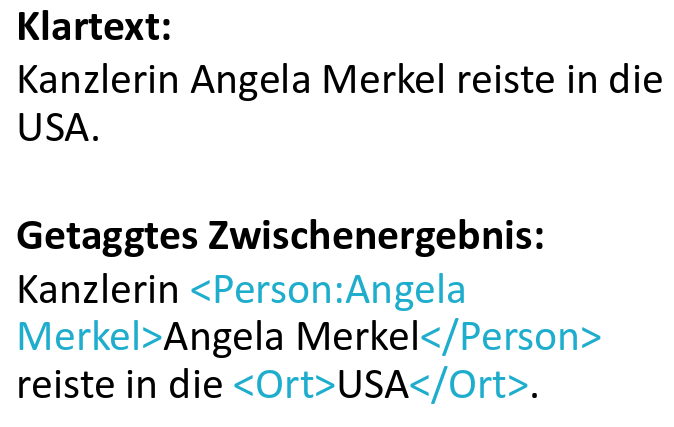
\includegraphics[scale=0.2]{Bild}
			\label{Bild}
			\caption{Vergleich Klartext und markierten Satz}
			\end{figure}

	\subsection{Erstellung der Traningsdaten}
		Das im vorherigem Abschnitt erwähnte, getaggte Dokument wurde zunächst in einzelne Wörter aufgeteilt.
		Dafür wurde der von der Stanford Core NLP mitgelieferte Tokenizer benutzt.
		Dieser transformiert den Text, sodass anschließend jede Zeile ein Wort (oder Satzzeichen) aufweist.
		Anschließend wurde der tokenisierte Text entsprechend des NER-Formats markiert. 
		Die XML-Tags wurden ausgelesen und alle Wörter innerhalb dieser Tags mit dem entsprechendem Label (z.B: 'PERSONEN' für Personen-Namen) versehen. 
		Alle anderen Wörter wurden mit 'O' markiert.
		Die daraus resultierende Tabelle speichert das Programm in der Datei ''TrainingsData.out'.


	\subsection{Erstellung des Klassifikators}
		Nachdem die Trainingsdaten maschinell erstellt wurden, konnte der Stanford NER trainiert.
		In unserem Programm wird die Main-Methode des Stanford NER Klassifikators aufgerufen und eine Propertydatei\footnote{in unseren Tests unter anderem ''Ressourcen/default.prop''} übergeben.
		Diese Propertydatei gibt Eigenschaften des Trainings und des zu erstellenden Klassifikators an.

		Für unsere Tests wählten wir zwei verschiedenen Property-Dateien.
		Zum einen die Property-Datei, welche in den FAQ der Stanford NER Webseite vorgestellt wird\footnote{vgl. ''default.prop''}, zum anderen die Propertydatei des deutschen Klassifikators ''German-Classifier-DEWAC''\footnote{vgl. ''german.dewac\_175m\_600.prop''}.
		Die Letztere weist für die deutsche Sprache angepasste Features auf und trainiert unter anderem zweimal auf den Trainingsdaten.

\section{Probleme innerhalb des Projekts}
\label{Probleme}
	Die Schwierigkeiten des Auffindens von zu markierenden Wörtern, sowie der Vermeidung von falsch-positiven Markierungen wurden bereits im Abschnitt 'Einlesen des Klartextes und Tagging' angesprochen. Dies war eines der größten Probleme innerhalb dieses Projekts und die Lösungsfindung sehr zeitaufwendig.

	Beim Extrahieren des Klartextes aus den gefilterten Artikeln mit dem Programm ''WikiExtraktor.py'' werden bei den einzelnen Artikeln Teile des Textes verworfen.
	Die Ursache war nicht genau ermittelbar. Vermutlich hängt dies jedoch mit der Länge des Textes zusammen, sodass Artikel nach einer bestimmten Länge abgeschnitten werden. Die Relevanz des Problems ist jedoch nicht weiter groß, da das Fehlen von Text einfach mit der Extraktion von weiteren Artikeln kompensiert werden kann.
	
	Zusätzlich war für die Evaluierung der Ergebnisse die Größe der Eingabedaten in den Trainer problematisch. Deswegen mussten wir uns auf eher kleine Mengen von ca. 150 getaggten Wikipedia-Artikeln (ca. 8MB Größe) beschränken, da größere Mengen deutlich länger dauern und mehr RAM-Speicher benötigen.
\section{Ergebnisse}
	Alle maschinell erstellten Klassifizierer wurden auf einem per Hand annotierten Goldstandart verglichen.
	Dieser Goldstandart bestand aus 100 Beispielsätzen (1530 Wörter und Satzzeichen) aus Nachrichtenartikeln oder Beispielsätzen des Projektes ''Wortschatz'' der Universität Leipzig.
	Des Weiteren haben wir unsere Klassifikator mit dem auf der Stanford NER Webseite erhältlichen deutschen Klassifikator verglichen.
	Die ausführlichen Ergebnisse sind in der \autoref{Ergebnistabelle} im Anhang zu finden.

	Aus den Ergebnissen kann man entnehmen, dass die Variante, welche die Personennamen trennt, einen deutlich besseren Recall-Wert aufweist.
	Dies ist dadurch zu erklären, dass im Text auch Personen markiert werden, welche nur mit Vor- oder Nachnamen erwähnt sind.
	Andererseits weist diese Variante ein schlechteres Ergebnis in der Genauigkeit (Precision) auf, da viele der Personennamen mehrdeutig sind (siehe \ref{Probleme} Probleme).

	Im Vergleich der benutzten Property-Dateien schneidet die Property-Datei des deuschen Klassifizierers besser ab.
	Die Unterschiede sind jedoch marginal (maximal 2,5\%).

	Bei der Analyse der einzelnen Kategorien fällt auf, dass das Markieren der Organisationen am schlechtesten abschneidet.
	Das ist zum Teil damit zu begründen, dass das Wörterbuch keine Abkürzungen (z.B. für Parteien) enthält.
	Dadurch wird der NER nicht mit diesen Abkürzungen trainiert und erkennt diese folglich nicht.

	Im Vergleich zu dem bereits existierenden Klassifikator\footnote{\url{http://www.nlpado.de/~sebastian/software/ner_german.shtml}} schneiden unsere Ergebnisse schlechter ab.
	Dies war jedoch zu erwarten, da es sich bei dem deutschen Klassifikator nach eigenen Aussagen um einen der Besten für die deutsche Sprache handelt.

\section{Fazit}
	Das maschinelle Erstellen von Trainigsdaten für den Stanford NER ist keine triviale Aufgabe.
	Unser Ansatz beruhte auf der Erstellung von Trainingsdaten mit Hilfe von Wörterbüchern.
	Diese Methodik bringt bestimmte Probleme mit sich.
	Besonders die Mehrdeutigkeit von Namen können mit diesem Verfahren schlecht gelöst werden.
	Außerdem ist das Wörterbuch niemals vollständig, sodass nicht alle Entitäten gefunden werden können.
	Vermutlich würde ein Einbezug des Kontextes eines Wortes eine Verbesserung mit sich bringen.


\newpage
\appendix{
\section{Anhang}
\hvFloat[%
nonFloat=true,%
capWidth=w,%
capPos=t,%
rotAngle=90,%
objectPos=c%
]{table}{%
\renewcommand{\arraystretch}{2}
\begin{tabular}{|c|c|c|c|c|c|c|c|c|}
\hline
Anzahl Artikel pro Kategorie & Variante & Property Datei & Precision & Recall & F1 & TP & FP & FN  \\
\hline
je 20 & Personenname getrennt & default & 40,80\% & 46,07\% & 43,27\% & 82& 119 & 96\\
\hline
je 20 & Personen Vollnamen & default & 52,53\% & 29,21\% & 37,55\% & 52 & 47 & 126\\
\hline
je 20 & Personenname getrennt & german.dewac\_175m\_600 & 40,72\% & 44,38\% & 42.47\% & 79 & 115 & 99\\
\hline
je 20 & Personen Vollnamen & german.dewac\_175m\_600 & 53,06\% & 29,21\% & 37,68\% & 52 & 46 & 126\\
\hline
\hline
je 50 & Personenname getrennt & default & 39,11\% & 44,38\% & 41,58\% & 79 & 123 & 99 \\
\hline
je 50 & Personen Vollname & default & 49,53\% & 29,78\% & 37,19\% & 53 & 54 & 125 \\
\hline
je 50 & Personenname getrennt & german.dewac\_175m\_600 & 40,98\% & 47,19\% & 43,86\% & 84 & 121 & 94 \\
\hline
je 50 & Personen Vollnamen & german.dewac\_175m\_600 & 50,94\% & 30,34\% & 38,03\% & 54 & 52 & 124 \\
\hline
\hline
  &  & German-Classifier-DEWAC & 65,81\% & 57,30\% & 61,26\% & 102 & 53 & 76 \\
\hline
  &  & German-Classifier-HGC & 61,22\% & 50,56\% & 55,38\% & 90 & 57 & 88 \\
\hline
\end{tabular}
}{Ergebnisse}{Ergebnistabelle}

\begin{table}
\centering
	\caption{150 Artikel, default Property, Personen generalisiert}
	\label{defPropGeneralisiert}
	\renewcommand{\arraystretch}{1,5}
	\begin{tabular}{|c|c|c|c|c|c|c|}
		\hline
		Entität & Precision & Recall & F1 & TP & FP & FN \\
		\hline
		ORGANISATION & 25,00\% & 5,13\% & 8,51\% & 2 & 6 & 37 \\
		\hline
		ORT & 50,67\% & 52,05\% & 51,35\% & 38 & 37 & 35 \\
		\hline
		PERSON & 54,17\% & 19,70\% & 28,89\% & 13 & 11 & 53 \\
		\hline
	\end{tabular}
\end{table}


\begin{table}
	\centering
	\caption{150 Artikel, default Property, Personen als Person}
	\renewcommand{\arraystretch}{1,5}
	\label{defPropPaP}
	\begin{tabular}{|c|c|c|c|c|c|c|}
		\hline
		Entität & Precision & Recall & F1 & TP & FP & FN \\
		\hline
		ORGANISATION & 25,00\% & 5,13\% & 8,51\% & 2 & 6 & 37 \\
		\hline
		ORT & 58,21\% & 53,42\% & 55,71\% & 39 & 28 & 34 \\
		\hline
		PERSON & 29,92\% & 57,58\% & 39,38\% & 38 & 89 & 28 \\
		\hline
	\end{tabular}
\end{table}

\begin{table}
	\centering
	\caption{150 Artikel, dewiki Property, Personen Generalisiert}
	\renewcommand{\arraystretch}{1,5}
	\label{dewacPropPG}
	\begin{tabular}{|c|c|c|c|c|c|c|}
		\hline
		Entität & Precision & Recall & F1 & TP & FP & FN \\
		\hline
		ORGANISATION & 25,00\% & 5,13\% & 8,51\% & 2 & 6 & 37 \\
		\hline
		ORT & 52,05\% & 52,05\% & 52,05\% & 38 & 35 & 35 \\
		\hline
		PERSON & 56,00\% & 21,21\% & 30,77\% & 14 & 11 & 52 \\
		\hline
	\end{tabular}
\end{table}


\begin{table}
	\centering
	\caption{150 Artikel, dewac Property, Personen als Person}
	\renewcommand{\arraystretch}{1,5}
	\label{dewacPropPaP}
	\begin{tabular}{|c|c|c|c|c|c|c|}
		\hline
		Entität & Precision & Recall & F1 & TP & FP & FN \\
		\hline
		ORGANISATION & 25,00\% & 5,13\% & 8,51\% & 2 & 6 & 37 \\
		\hline
		ORT & 56,72\% & 52,05\% & 54,29\% & 39 & 29 & 35 \\
		\hline
		PERSON & 33,85\% & 66,67\% & 44,90\% & 44 & 86 & 22 \\
		\hline
	\end{tabular}
\end{table}


\end{document}
